\documentclass[a4paper]{article}

\setlength{\parindent}{0pt}
\setlength{\parskip}{1em}

\pagestyle{headings}

\usepackage{amssymb}
\usepackage{amsmath}
\usepackage{amsthm}
\usepackage{mathtools}
\usepackage{graphicx}
\usepackage{hyperref}
\usepackage{color}
\usepackage{microtype}
\usepackage{tikz}
\usepackage{pgfplots}
\usepackage{pgfplotstable}

\newcommand{\N}{\mathbb{N}}
\newcommand{\Q}{\mathbb{Q}}
\newcommand{\Z}{\mathbb{Z}}
\newcommand{\R}{\mathbb{R}}
\newcommand{\C}{\mathbb{C}}
\newcommand{\D}{\mathcal{D}}
\renewcommand{\S}{\mathcal{S}}
\renewcommand{\P}{\mathbb{P}}
\newcommand{\F}{\mathbb{F}}
\newcommand{\E}{\mathbb{E}}
\newcommand{\bra}{\langle}
\newcommand{\ket}{\rangle}


\graphicspath{{Image/}}

\hypersetup{
    colorlinks=true,
    linktoc=all,
    linkcolor=blue
}

\theoremstyle{definition}
\newtheorem*{axiom}{Axiom}
\newtheorem*{claim}{Claim}
\newtheorem*{conv}{Convention}
\newtheorem*{coro}{Corollary}
\newtheorem*{defi}{Definition}
\newtheorem*{eg}{Example}
\newtheorem*{lemma}{Lemma}
\newtheorem*{notation}{Notation}
\newtheorem*{prob}{Problem}
\newtheorem*{post}{Postulate}
\newtheorem*{prop}{Proposition}
\newtheorem*{rem}{Remark}
\newtheorem*{thm}{Theorem}

\DeclareMathOperator{\vdiv}{div}
\DeclareMathOperator{\grad}{grad}
\DeclareMathOperator{\curl}{curl}
\DeclareMathOperator{\Ann}{Ann}
\DeclareMathOperator{\Fit}{Fit}
\DeclareMathOperator{\Diag}{Diag}
\DeclareMathOperator{\tr}{tr}
\DeclareMathOperator{\im}{im}
\DeclareMathOperator{\Mat}{Mat}
\DeclareMathOperator{\Log}{Log}
\DeclareMathOperator{\Isom}{Isom}
\DeclareMathOperator{\Mesh}{Mesh}
\DeclareMathOperator{\Sym}{Sym}
\DeclareMathOperator{\Aut}{Aut}
\DeclareMathOperator{\cosech}{cosech}
\DeclareMathOperator{\Card}{Card}
\DeclareMathOperator{\Gal}{Gal}


\setcounter{section}{-1}

\begin{document}

\title{Quantum Computation}

\maketitle

\newpage

\tableofcontents

\newpage

\section{Introduction}
asdasd

\newpage

Exercise classes: Sat 3 Nov 11am MR4, Sat 24 Nov 11am MR4, early next term (tba).\\
Thursday 8 November lecture is moved to Saturday 10 November 11am (still MR4).

---Lecture 2---

\section{1}

Recall that we have an oracle $U_f$ for $f:\Z_M \to \Z_\N$ periodic, with period $r$, $A=M/r$. We want to find $r$ in $O(poly(m))$ time where $m=\log M$.

\subsection{The quantum algorithm}
Work on state space $\mathcal{H}_M \otimes \mathcal{N}$ with basis $\{|i\ket |k\ket\}_{i \in \Z_M, k \in \Z_N}$.\\
$\bullet$ Step 1. Make staet $\frac{1}{\sqrt{M}}\sum_{i=0}^{M-1} |i\ket|0\ket$.\\
$\bullet$ Step 2. Apply $U_f$ to get $\frac{1}{\sqrt{M}} \sum_{i=0}^{M-1} |i\ket |f(i)\ket$.\\
$\bullet$ Step 3. Measure the 2nd register to get a result $y$. By Born rule, the first register collapses to all those $i$'s (and only those) with $f(i)$ equal to the seen $y$, i.e. $i=x_0,x_0+r,...,x_0+(A-1)r$, where $0 \leq x_0 < r$ in 1st period has $f(m)=y$.\\
Discard 2nd register to get $|per\ket = \frac{1}{\sqrt{A}} \sum_{j=0}^{A-1}|x_0+jr\ket$.\\
Note: each of the $r$ possible function values $y$ occurs with same probability $1/r$, so $0 \leq x_0 < r$ has been chosen uniformly at random.\\
If we now measure $|per\ket$, we'd get a value $x_0+jr$ for uniformly random $j$, i.e. random element $(x_0^{th})$ of a random period $(j^{th})$, i.e. random element of $\Z_m$, so we could get no information about $r$.\\
$\bullet$ Step 4. Apply quantum Fourier transform mod $M$ (QFT) to  $|per\ket$. Recall the definition of QFT: $QFT: |x\ket \to \sum_{y=0}^{M-1} \omega^{xy} |y\ket$ for all $x \in \Z_M$ where $\omega = e^{2\pi i/M}$ is the $M$th root of unity. The existing result is that QFT mod $M$ can be implemented in $O(M^2)$ time.\\
Then we get 
\begin{equation*}
    \begin{aligned}
    QFT |per\ket &= \frac{1}{\sqrt{MA}} \sum_{j=0}^{A-1} \left(\sum_{y=0}^{M-1} \omega^{(x_0+jr)y}|y\ket\right)\\
    &= \frac{1}{\sqrt{MA}} \sum_{y=0}^{M-1} \omega^{x_0y} \left[\sum_{j=0}^{A-1} \omega^{jry}\right] |y\ket \ (*)
    \end{aligned}
\end{equation*}
where we group all the terms with the same $|y\ket$ together. One good thing is that the sum inside the square bracket is a geometric series, with ratio $\alpha = \omega^{ry} = e^{2\pi iry/M} = (e^{2\pi i/A})^y$.\\
Hence term inside bracket $=A$ if $\alpha=1$, i.e. $y=kA = k \frac{M}{r}$, $k=0,1,...,(r-1)$, and equals $0$ otherwise when $\alpha \neq 1$. Now\\
\begin{equation*}
    \begin{aligned}
        QFT |per\ket = \sqrt{\frac{A}{M}} \sum_{k=0}^{r-1} \omega^{x_0 k \frac{M}{r}} |k \frac{M}{r}\ket
    \end{aligned}
\end{equation*}
The random shift $x_0$ now appears only in phase, so measurement probabilities are now independent of $x_0$!

Measuring $QFT |per\ket$ gives a value $c$, where $c = k_0 \frac{M}{r}$ with $0 \leq k_0 \leq r-1$ chosen uniformly at random. Thus $\frac{k_0}{r} = \frac{c}{M}$, note that $c,M$ are known, $r$ is unknown (what we want), and $k_0$ is unknown but uniformly random.

So note that if we are lucky and get a $k_0$ that is coprime to $r$ then we could just simplify $\frac{c}{M}$ to get $r$. Obviously we cannot be always lucky every time, but by theorem in number theory, the number of integers $<r$ coprime to $r$ grows as $O(r/\log\log r)$ for large $r$, so we know probability of $k_0$ coprime to $r$ is $O(\frac{1}{\log\log r})$.

Then by some probability calculation we know that $O(1/p)$ trials are enough to achieve $1-\varepsilon$ probability of success.

So afer Step 4, cancel $c/M$ to the lowest terms $a/b$, giving $r$ as denominator $b$ (if $k_0$ is coprime to $r$). Check $b$ value by computing $f(0)$ and $f(b)$, since $b=r$ iff $f(0) = f(b)$.

Repeating $K=O(\log\log r)$ times gives $r$ with any desired probability.

Further insights into utility of QFT here:\\
Write $R = \{0,r,2r,...,(A-1)r\} \subseteq \Z_M$. $|R\ket = \frac{1}{\sqrt{A}} \sum_{k=0}^{A-1} |kr\ket$, and $|per\ket = |x_0 + R\ket = \frac{1}{\sqrt{A}} \sum_{k=0}^{A-1} |x_0+br \ket$ where $x_0$ is the random shift that caused problem previously.\\
For each $x_0 \in \Z_M$, consider mapping $k \to k+x_0$ (shift by $x_0$) on $\Z_M$, which is a 1-1 invertible map.

So linear map $U(x_0)$ on $\mathcal{H}_M$ defined by $U(x_0): |k\ket \to |k+x_0\ket$ is unitary, and $|x_0+R \ket = U(x_0) |R\ket$.

Since $(\Z_M,+)$ is abelian, $U(x_0)U(x_1) = U(x_0+x_1) =U(x_1)U(x_0)$ i.e. all $U(x_0)$'s commute as operators on $\mathcal{H}_M$.\\
So we have orthonormal basis of common eigenvectors $|\chi_k\ket\}_{k \in \Z_M}$, called \emph{shift invariant states}.

$U(x_0)|\chi_k\ket = \omega(x_0,k)|\chi_k\ket$ for all $x_0,k \in \Z_M$ with $|\omega(x_0,k)| = 1$. Now consider $|R\ket$ written in $|\chi\ket$ basis,\\
$|R\ket = \sum_{k=0}^{M-1} a_k | \chi_k\ket$ where $a_k$'s depending on $r$ (not $x_0$).\\
Then $|per\ket = U(x_0) |R\ket = \sum_{k=0}^{M-1}a_k \omega(x_0,k) |\chi_k\ket$, and measurement in the $\chi$-basis has $prob(k) = |a_k \omega(x_0,k)|^2 = |a_k|^2$ which is independent of $x_0$, i.e. giving information about $r$!

---Lecture 3---



Recall last time we had $\mathcal{H}_M$: shift operations $U(x_0) |y \ket = |y+x_0\ket$ for $x_0,y \in \Z_M$, which all permute, so have a common eigenbasis (shift invariant states) $\{|\chi_k\ket \}_{k \in \Z_M}$, $U(x_0) | x_k\ket = \omega(x_0,k) |\chi_k\ket$.\\
Measurement of $|x_0+R \ket = \frac{1}{\sqrt{A}} \sum_{l=0}^{A-1} |x_0 + l_r \ket = U(x_0) |R\ket$ in $|\chi\ket$ basis has output distribution independent of $x_0$, therefore gives information about $r$.

Introduce QFT as the unitary mapping that rotates $\chi$-basis to standard basis, i.e. define $QFT|\chi_k \ket = |k\ket$. So QFT followed by measurement implements $\chi$-basis measurement.

Explicit form of $|\chi_k\ket$ eigenspaces (!): consider
\begin{equation*}
    \begin{aligned}
        |\chi_k\ket = \frac{1}{\sqrt{M}}\sum_{l=0}^{M-1} e^{-2\pi i kl/M}|l\ket
    \end{aligned}
\end{equation*}
Then
\begin{equation*}
    \begin{aligned}
        U(x_0) |\chi_k \ket &= \frac{1}{\sqrt{M}} \sum_{l=0}^{M-1} e^{-2\pi i kl/M}|l+x_0\ket \\
        &= \frac{1}{\sqrt{M}} \sum_{\tilde{l}=0}^{M-1} e^{-2\pi i k (\tilde{l}-x_0)/M} | \tilde{l} \ket \text { where } \tilde{l} = l+x_0\\
        &= e^{2\pi i k x_0 / M} \cdot |\chi_k\ket
    \end{aligned}
\end{equation*}
i.e. these are the shift invariant staets, eigenvalues $\omega(x_0,k) = e^{2\pi i k x_0/M}$.

Matrix of QFT: So
\begin{equation*}
    \begin{aligned}
        [QFT^{-1}]_{lk} = \frac{1}{\sqrt{M}} e^{-2\pi i lk/M}
    \end{aligned}
\end{equation*}
(componets of $|\chi_k \ket = QFT^{-1} |k\ket$ as $k^{th}$ column). So
\begin{equation*}
    \begin{aligned}
        [QFT]_{kl} = \frac{1}{\sqrt{M}} e^{2\pi i lk / M}
    \end{aligned}
\end{equation*}
as expected.

\newpage

\section{The hidden subgroup problem (HSP)}

Let $G$ be a finite group of size $|G|$. Given (oracle for) function $f:G \to X$ ($X$ is some set), and promise that there is a subgroup $K < G$ such that $f$ is constant on (left) cosets of $K$ in $G$, and $f$ is distinct on distinct cosets.\\
The problem: determine the \emph{hidden subgroup} $K$ (e.g. output a set of generators, or sample uniformly from $K$).\\
We want to solve in time $O(poly(\log |G|))$ (an efficient algorithm) with any constant probability $1-\varepsilon$.

Examples of problems that can be cast(?) as HSPs:\\
(i) periodicity: $f:\Z_M \to X$, periodic with period $r$. Let $G=(\Z_m,+)$, the hidden subgroup is $K=\{0,r,2r,...\} < G$, cosets $x_0+K = \{x_0,x_0+r,x_0+2r,...\}$. The period $r$ is generator of $K$.\\
(ii) discrete logarithm: for prime $p$, $\Z_p^* = \{1,2,...,p-1\}$ with multiplication mod $p$. $g \in \Z_p^*$ is a generator (or primitive root mod $p$). If powers generate all of $\Z_p^*$, $\Z_p^* = \{g^0 = 1,g^1,...,g^{p-2}\}$, then also $g^{p-1} \equiv 1 \pmod p$ (easy number theory).\\
Fact: the generator always exists if $p$ is prime. So any $x \in \Z_p^*$ can be written $x = g^y$ for some $y \in \Z_{p-1}$, write $y=\log_g x$ called the discrete log of $x$ to base $g$.

Discrete log problem: given a generator $g$ and $x \in \Z^*_p$, compute $y=\log_g x$ (classically hard).\\
To express as HSP, consider $f:\Z_{p-1} \times \Z_{p-1} \to \Z_p^*$: $f(a,b) = g^a x^{-b} \ mod \ p = g^{a-yb} \ mod \ p$.\\
Then check: $f(a_1,b_1) = f(a_2,b_2)$ iff $(a_2,b_2) = (a_1,b_1)+\lambda(y,1)$ where $\lambda \in \Z_{p-1}$.

So if $G = \Z_{p-1} \times \Z_{p-1}$, $K=\{\lambda(y,1):\lambda \in \Z_{p-1}\} < G$. Then $f$ is constant and distinct on the cosets of $K$ in $G$, and generator $(y,1)$ gives $y=\log_g x$.\\

(iii) graph problems ($G$ non-abelian now): consider undirected graph $A = \{V,E\}$, $|V| =n$, with at most one edge between any two vertices. Label vertices by $[n] = \{1,2,...,n\}$.\\
Introduce the permutation group $\mathcal{P}_n$ of $[n]$. Define $Aut(A)$ to be the group of automorphisms of $A$, which is a subgroup of $\mathcal{P}_n$, containing exactly the permutations $\pi \in \mathcal{P}_n$ such that for all $i,j \in [n]$, $(i,j) \in E \iff (\pi(i),\pi(j)) \in E$, i.e. the labelled graph $\pi(A)$ obtained by permuting labels of $A$ by $\pi$ is the same \emph{labelled} graph as $A$.

Associated HSP: Take $G = \mathcal{P}_n$. Let $X$ be set of all labelled graphs on $n$ vertices. Given $A$, consider $f_A: \mathcal{P}_n \to X$ by $f_A(\pi) = \pi(A)$, $A$ with labels permuted by $\pi$. The associated hiiden subroup is $Aut(A) = K$.

Application: if we can sample uniformly from this $K$, then we can solve graph isomorphism problem (GI): two labelled graphs $A,B$ are isomorphic if there is 1-1 map $\pi:[n] \to [n]$ such that for all $i,j \in [n]$, $i,j$ is an edge in $A$ iff $\pi(i),\pi(j)$ is an edge in $B$, i.e. $A$ and $B$ are the same graph but just labelled differently.

---Lecture 4---

Let's come back to the graph isomorphism problem.

Problem: given $A,B$, decide if $A \cong B$ or not. This can be expressed as anon-abelian HSP (on example sheet), no known classical polynomial time algorithm. However it is in NP, but it is not believed to be NP-complete.\\
Recent result (2017): a quasi-poly time classical algorithm (L.Babai).

Quantum algorithm for finite \emph{abelian} HSP:\\
Write group $(G,+)$ additively.

Construction of shift invariant states and FT for $G$:\\
Let's introduce some representation theory for abelian group $G$. Consider mapping $\chi:G \to \C^* = (\C \setminus \{0\}, \cdot)$ satisfying $\chi(g_1+g_2) = \chi(g_1)\chi(g_2)$, i.e. $\chi$ is a group homomorphism. Such $\chi$'s are called \emph{irreducible} representations of $G$.\\
We have the following properties (without proof), which we'll call Theorem A later when we refer to it:\\
(i) any value $\chi(g)$ is a $|G|^{th}$ root of unity (so $\chi$: $G \to S^1$ = unit circle in $\C$);\\
(ii) (Schur's lemma, orthogonality): If $\chi_i$ and $\chi_j$ are representations, then $\sum_{g \in G} \chi_i (g) \bar{\chi}_j(g) =\delta_{ij}|G|$;\\
(iii) there are always exactly $|G|$ different representations $\chi$ (well, this is a special case of general representation theory).

By (iii), we can label $\chi$'s as $\chi_g$ for $g \in G$. For example, $\chi(g) = 1$ for all $g \in G$ is always an irreducible representation (the trivial representation), labelled $\chi_0$;\\
Then by orthogonality (ii) for any $\chi \neq \chi_0$ gives $\sum_{g \in G} \chi(g) = 0$.

Shift invariant states: in space $\mathcal{H}_{|G|}$ with basis $\{|g\ket\}_{g \in G}$, introduce \emph{shift operators} $U(k)$ for $k \in G$ defined by $U(k): |g\ket \to |g+k\ket$. Clearly these all commute, so there is simultaneous eigenbasis:\\
For each $\chi_k$, $k\in G$, consider state $|\chi_k \ket = \frac{1}{\sqrt{|G|}} \sum_{g \in G} \bar{\chi}_k (g)|g\ket$. Then theorem A(ii) implies these form orthonormal basis, and $U(g) |\chi_k\ket = \chi_k(g)|\chi_k\ket$.
\begin{proof}
    \begin{equation*}
        \begin{aligned}
            U(g)|\chi_k\ket &= \frac{1}{\sqrt{|G|}} \sum_{h \in G} \bar {\chi_k(h)} |h+g\ket\\
            &\stackrel{h'=h+g}{=} \frac{1}{\sqrt{|G}} \sum_{h' \in G} \bar{\chi_k(h'-g)} |h' \ket
        \end{aligned}
    \end{equation*}
    This implies that 
    \begin{equation*}
        \begin{aligned}
            \chi_k*-g) = (\chi_k(g))^{-1} = \bar{\chi_k(g)},\\
            \bar{\chi_k(h'-g)} = \bar{\chi_k(h')}\bar{\chi_k(-g)} = \chi_k(h')\chi_k(g)
        \end{aligned}
    \end{equation*}
    So
    \begin{equation*}
        \begin{aligned}
            U(g) | \chi_k \ket = \frac{1}{\sqrt{|G|}} = \sum_{h' \in G} \chi_k(g) \bar{\chi}_k (h') | h' \ket = \chi_k (g) | \chi_k \ket
        \end{aligned}
    \end{equation*}
\end{proof}

So $|\chi_k \ket$'s are common eigenspaces, called \emph{shift-invariant states}.\\
    Introduce (define) Fourier transform QFT for group $G$ as the unitary that $QFT|\chi_g\ket = |g\ket$ for all $g \in G$.\\
    In $|g\ket-$basis matrices, $k^{th}$ column of $(QFT^{-1}) = $components of $|\chi_k\ket$, i.e. $\frac{1}{\sqrt{|G|}} \bar{\chi_k}(g) = [QFT^{-1}]_{gk}$.\\
    So $[QFT]_{kg}^\dagger = \frac{1}{\sqrt{|G|}}\chi_k(g)$, and so $QFT|g\ket = \frac{1}{\sqrt{|G|}} \sum_{k \in G} \chi_k (g) |k\ket$.

\begin{eg}
    $G=\Z_M$. Check $\chi_a(b) = e^{2\pi iab/M}$, $a,b \in \Z_M$ is a representation.\\
    Similarly, for $G=\Z_{M_1} \times ... \times \Z_{M_r}$, $(a_1,...,a_r) = g_1, (b_1,...,b_r) = g_2$ where $g_1,g_2 \in G$, $$\chi_{g_1}(g_2) \stackrel{def}{=} e^{2\pi i \left(\frac{a_1b_1}{M_1} + ... + \frac{a_rb_r}{M_r}\right)}$$ is a representation of $G$. And we get $$QFT_G =QFT_{M_1} \otimes ... \otimes QFT_{M_r}$$ on $\mathcal{H}_{|G|} = \mathcal{H}_{M_1} \otimes ... \otimes \mathcal{H}_{M_r}$.\\
    This is exhaustive, since by classification theorem, every finite abelian group $G$ is isomorphic to a direct product of the form $G \cong \Z_{M_1} \times ... \times \Z_{M_r}$. Furthermore, we can insist that $M_i$ are prime powers $p_i^{s_i}$, where $p_i$ are not necessarily distinct.
\end{eg}

Quantum algorithm for finite abelian HSP:\\
Let $f:G \to X$, hidden subgroup $K<G$. We have cosets $K=0+K,g_2+K,...,g_m+K$, where $m=|G|/|K|$. State space as usual, with basis $\{|g\ket, |x\ket \}_{g \in G, x \in X}$.\\
$\bullet$ make the state $\frac{1}{\sqrt{|G|}} \sum_{g \in G} |g\ket |0\ket$;\\
$\bullet$ Apply oracle $U_f$, get $\frac{1}{\sqrt{|G|}} \sum_{g \in G} |g\ket |f(g)\ket$;\\
measure second register to see a value $f(g_0)$.\\
Then first register gives coset state (remember the function is constant on each coset). $|g_0+K \ket = \frac{1}{\sqrt{|K|}} \sum_{k \in K} |g_0 + K \ket = U(g_0) |K\ket$.\\
Apply QFT and measure to obtain result $g \in G$.

---Lecture 5---

Last time we disccused how to solve the abelian HSP problem. Now how does the output $g$ related to $K$?\\
$\bullet$ the output distribution of $g$ is independent of $g_0$, so same as that obtained from $QFT|K \ket$ (i.e. $g_0 = 0$) since:\\
write $|K \ket $ in shift invariant basis $|\chi_g \ket$'s, $|K\ket = \sum_{g} a_g | \chi_g \ket$, then $|g_0+K \ket = U(g_0) |K\ket = \sum a_g \underbrace{\chi_g(g_0) | \chi_g \ket}_{ = U(g_0) | \chi_g \ket}$; but $QFT|\chi_g \ket = |g\ket$, so $Prob(g) = |a_g \chi_g (g_0)|^2 = |a_g|^2$ as $\chi_g(g_0)| = 1$.

Thus look at $QFT|K \ket$. Recall $QFT|k \ket = \frac{1}{\sqrt{|G|}} \sum_{l \in G} \chi_l(k) |l\ket$, so $QFT |K\ket = \frac{1}{\sqrt{|G|}} \frac{1}{\sqrt{|K|}} \sum_{l \in G} \left[\sum_{k \in K} \chi_l(k) \right] |l\ket$.\\
The terms in $[...]$ involves irreducible representation $\chi_l$ of $G$ restricted to subgroup $K < G$, which is an irreducible representation of $K$. Hence 
\begin{equation*}
    \begin{aligned}
        \sum_{k \in K} \chi_l(k) = \left\{
            \begin{array}{ll}
                |K| & \chi_l \text{ restricts to trivial irreducible representation on } K\\
                0 & \text{ otherwise}
            \end{array}
        \right.
    \end{aligned}
\end{equation*}
and
$$QFT|K\ket = \sqrt{\frac{|K|}{|G|}} \sum_{l \in G \text{ with }\chi_l\text{ reducing to trivial irreducible representation of }K} |l\ket$$
So measurement gives a uniformly random choice of $l$ such that $\chi_l(k) = 1$  for all $k \in K$.\\
e.g. If $K$ has generators $k_1,k_2,...,k_M$, $M=O(\log |K|) = O(\log |G|)$, then output has $\chi_l(k_i) = 1$ for all $i$.

It can be shown that if $O(\log|G|)$ such $l$'s are chosen uniformly at random, then with probability $>2/3$ they suffice to determine a generating set for $K$ via equations $\chi_l(k) = 1$.\\
(see example sheet 1 for particular examples).

\begin{eg}
    If $G = \Z_{M_1} \times ... \times \Z_{M_q}$.\\
    We had for $l=(l_1,...,l_q)$, $g \in (b_1,...,b_q) \in G$,
    $$\chi_l(g) = e^{2\pi i (\frac{l_1k_1}{M_1} + ... + \frac{l_qb_q}{M_q})}$$
    So for $k=(k_1,...,k_q)$, $\chi_l(k) = 1$ becomes
    $$\frac{l_1k_1}{M_1} + ... + \frac{l_qk_q}{M_q} \equiv 0 \pmod 1$$
    (i.e. is an integer), a homogeneous linear equation on $K$, and $O(\log |K|)$ is independent such that equations determine $K$ as null space.
\end{eg}

Some remarks on HSP for non-abelian groups $G$ (write multiplicatively):\\
As before, can easily generate coset states 
$$ |g_0 K \ket = \frac{1}{\sqrt{|K|}} \sum_{k \in K} |g_0 K\ket$$
where $g_0$'s are randomly chosen. But problems arise with QFT construction, because now there's no basis of shift-invariant states exists! (this is since $U(g_0)$'s don't commute anymore, so no common full eigenbasis).

Construction of non-abelian Fourier Transform (some more representation theory):\\
$\bullet$ $d$-dimensional representation of $G$ is a group homomorphism $\chi: G \to U(d)$ where $U(d)$ is the space of $d \times d$ unitary matrices acting on $\C^d$, by $\chi(g_1 g_2) \chi(g_1)\chi(g_2)$. (see part II representation theory for the general form)\\
$\bullet$ $\chi$ is irreducible representation if no subspace of $\C^d$ is left invariant under $\chi(g)$ for all $g \in G$ (i.e. cannot simultaneously block diagonalise all $\chi(g)$'s by a basis change).\\
$\bullet$ a complete set of irreducible representation: set $\chi_1,...,\chi_m$ such that any irreducible representation is unitarily equivalent to one of them (equivalence $\chi \to \chi' = V\chi V^T$).

\begin{thm} (non-abelian version of theorem A -- properties of representations)\\
    If $d_1,...,d_m$ are dimensions of a complete set of irreducible representations $\chi_1,...,\chi_m$, then:\\
    (i) $d_1^2+...+d_m^2 = |G|$;\\
    (ii) Write $\chi_i(g)_{jk}$ for the $(j,k)^{th}$ entry of matrix $\chi_i(g)$, where $j,k = 1,...,d_i$. Then (Schur orthogonality):
    $$\sum_g \chi_i(g)_{jk} \bar{\chi}_{i'}(g)_{j'k'} = |G| \delta_{ii'} \delta{jj'}\delta{kk'}$$
    Hence states
    $$|\chi_{i,jk} \ket \equiv \frac{1}{\sqrt{|G|}} \sum_{g \in G} \bar{\chi}_i(g)_{jk} |g\ket$$
    is an orthonomal basis.
\end{thm}

$\bullet$ QFT on $G$ \emph{defined} to be the unitary that rotates $\{|\chi_{ijk}\ket\}$ basis into standard basis $\{|g\ket\}$. However, $|\chi_{ijk}\ket$ are \emph{not} shift invariant for all $U(g_0)$'s, and consequently measurement of coset state $|g_0 K\ket$ in $|\chi \ket$-basis gives an output distribution \emph{not} independent of $g_0$.

However, \emph{partial} shift invariance survives: Consider the incomplete measurement $M_{rep}$ on $|g_0 K\ket$ that distinguishes only the irreducible representations (i.e. $i$ values) and not all $(i,j,k)$'s.\\
i.e. with measurement outcome $i$ associated to $d_i^2$-dimensional orthogonal subspaces spanned by $\{|\chi_{(i),jk}\ket\}_{j,k = 1,...,d_i}$.\\
Then $\chi_i(g_1,g_2) = \chi_i(g_1) \chi_i(g_2)$ implies output distribution of $i$ values is independent of $g_0$, giving direct, albeit imcomplete, information about $K$.\\
E.g. conjugate subgroups $K$ and $ = g_0 K g_0^{-1}$ for some $g_0 \in G$ give \emph{same} output distribution.

---Lecture 6---\\
Non-abelian HSP/FT remarks:\\
For efficient HSP algorithm, we also need QFT to be efficiently implementable, i.e. $poly(\log|G|)$-time.\\
This is true for any abelian $G$ and some non-ablien $G$'s (such as $\mathcal{P}_n$), but even in latter case there's no known efficient HSP algorithm.

Some known result:\\
for normal subgroups, i.e. $gK= Kg$ for all $g \in G$:
\begin{thm} (Hallgrer, Russell, Tashma, SIAM J.Comp 32 p916-934 (2003))\\
    Suppose $G$ has efficient QFT. Then if hidden subgroup $K$ is normal, then there is an efficient HSP quantum algorithm.\\
    (Construct coset state $|g_0 K\ket$, perform $M_{rep}$ on it.)\\
    Repeat $O(\log|G|)$ times. Then $K$ normal implies outputs suffice to determine $K$.
\end{thm}

\begin{thm} (Ettinger, Hoyer, Knill)\\
    For general non-abelian HSP, $M=O(poly(\log|G|))$ random coset states $|g_1K\ket$,...,$g_M K\ket$ suffice to determine $K$ from $M$ coset states, but it's not efficient.\\
    See example sheet for a proof -- construct a measurement procedure on $|g_1K\ket \otimes ... \otimes g_MK\ket$ to determine $K$, but it takes exponential time in $\log|G|$.
\end{thm}

The phase estimation algorithm:\\
$\bullet$ a unifying principle for quantum algorithms, uses $QFT_{2^n}$ again.\\
$\bullet$ many applications, e.g. an alternative efficient factoring algorithm (A.Kitaev).

Given unitary operator $\mathcal{U}$ and eigenstate $|v_\phi \ket \cdot \mathcal{U} | v_{\phi}\ket = e^{2\pi i\phi} | v_\phi\ket$, we want to estimate phase $\phi$, where $0 \leq \phi < 1$ (to some precision, say to $n$ binary digits).

We'll need \emph{controlled-$U^k$} for integers $k$, writte $C-U^k$, which satisfies $c-U^k |0\ket |\xi\ket = |0\ket |\xi\ket$, $C-U^k |1\ket |\xi\ket = |1\ket U^k|\xi\ket$, where $|\xi\ket$ in general has dimension $d$.\\
Note $U^k |v_\phi\ket = e^{2\pi ik\phi} | v_\phi\ket$, $C-(U^k) = (C-U)^k$.

\begin{rem}
    Given $U$ as a formula or (arant?) description, we can readily implement $C-U$, e.g. just control each gate of $U$'s circuit.\\
    However, if $U$ is given as a \emph{black box}, we need further info:\\
    $\bullet$ it suffices to have an eigenstate $|\alpha\ket$ with known eigenvalue $U|\alpha\ket = e^{i\alpha} |\alpha\ket$:\\
    We can consider

    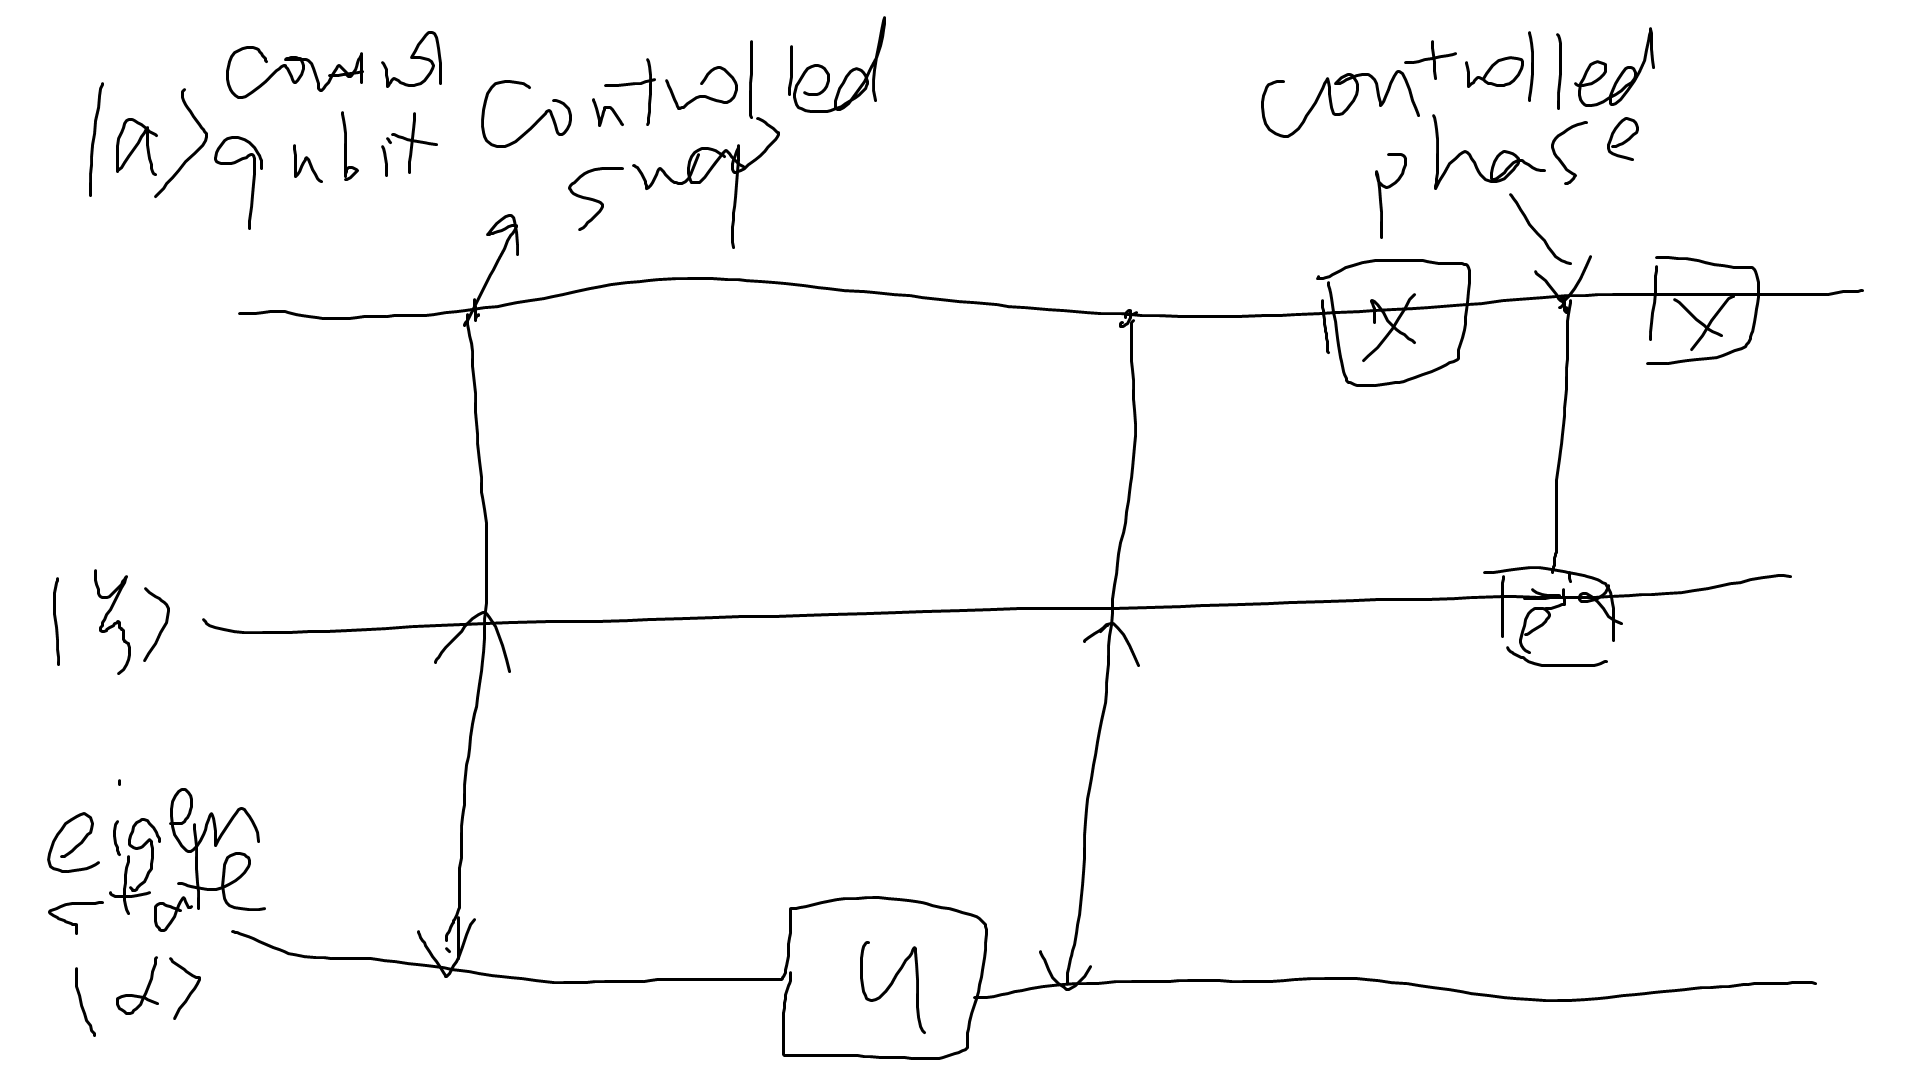
\includegraphics[scale=0.5]{image/QC_01.png}
    Where we get $CU|a\ket |\xi\ket$ at the first two row and the third row $|\alpha\ket$ is always unchanged.\\
    To see how it works, just check circuit action. (...)
\end{rem}

We'll actually want \emph{generalised controlled-$U$} with $|x\ket |\xi\ket \to |x\ket U^x |\xi\ket$, where $|x\ket$ has $n$ qubits, i.e. $x \in \Z_{2^n}$.\\
We can make this thing from $C-(U^k)$ as follows:

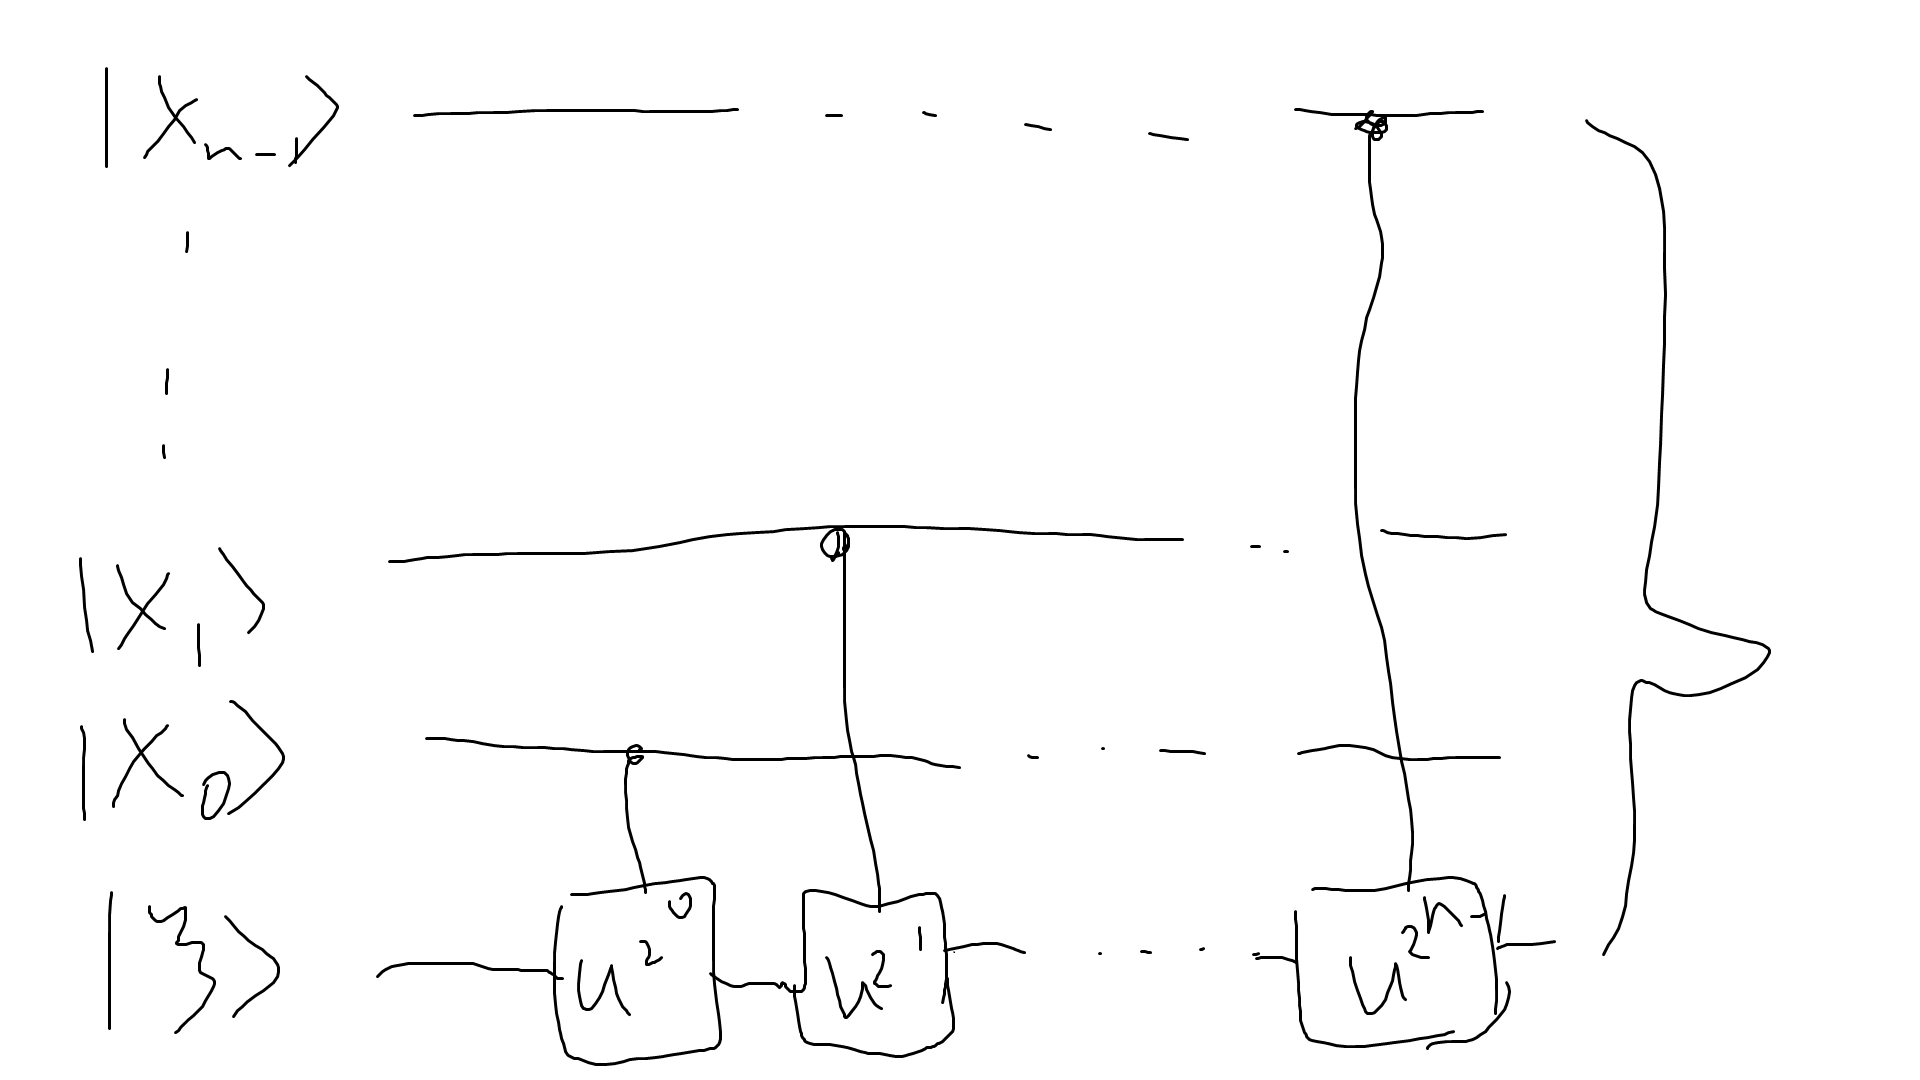
\includegraphics[scale=0.5]{image/QC_02.png}

We get $|x\ket U^x |\xi\ket$, where $x=x_{n-1}...x_1x_0$ binary, $U^x = U^{2^{x_{n-1}}} ... U^{2^{x_1}}U^{2^{x_0}}$.\\
Note: if input $|\xi\ket = |v_\phi\ket$, then get $e^{2\pi i \phi x}|v_\phi\ket$.

Now suppose over all $x=0,1,...,2^{n-1}$ and use $|\xi\ket = |v_\phi\ket$,

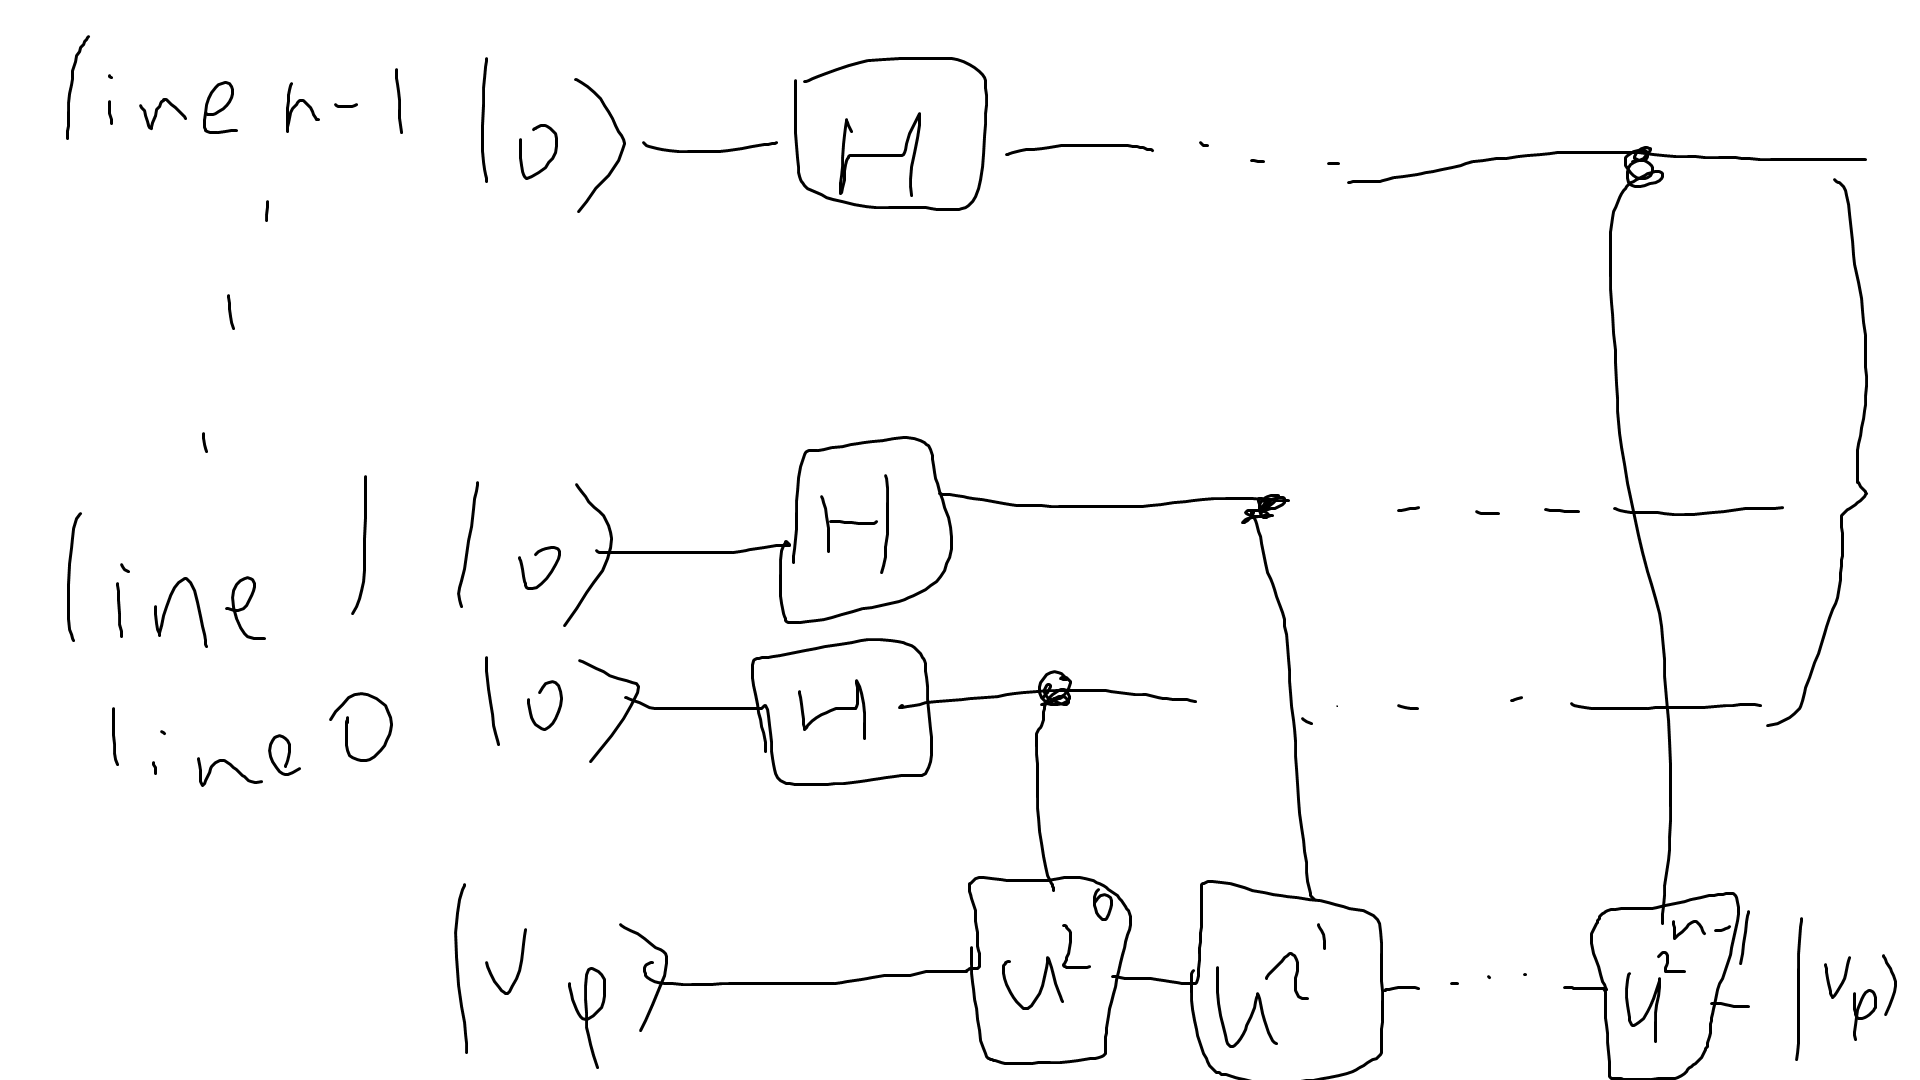
\includegraphics[scale=0.5]{image/QC_03.png}

Where the output is $\frac{1}{\sqrt{2^n}} \sum_x e^{2\pi i\phi x} |x\ket$, we call this state $|A\ket$.

Finally apply $QFT_{2^n}^{-1}$ to $|A\ket$ and measure to see $y_0,...,y_{n-1}$ on lines $0,1,...,n-1$. Then output $0.y_0...y_{n-1} = \frac{y_0}{2}+...+\frac{y_{n-1}}{2^{n-1}}$, as the estimate of $\phi$.\\
That's the phase estimation algorithm (for given $U$ and $V_\phi\ket$).

Suppose $\phi$ actually had only $n$ binary digits, i.e. $\phi$ exactly equals $0.z_0z_1...z_{n-1}$ for some $z_k=0,1$ for all $k$.

Then $\phi = \frac{z_0...z_{n-1}}{2^n} = \frac{z}{2^n}$ where $z$ is $n$-bit integer in $\Z_{2^n}$, and
$$ |A\ket = \frac{1}{\sqrt{2^n}} \sum_x e^{2\pi ixz/2^n} |x\ket$$
\emph{is} $QFT_{2^n}$ of $|z\ket$.\\
So $QFT^{-1} |A\ket = |z\ket$ and get $\phi$ exactly, with certainty.\\
In this case the algorithm up to (not including) final measurements is a unitary operation, mapping $|0\ket ... |0\ket |v_\phi \ket \to |z_0 \ket ... |z_{n-1} \ket |v_\phi\ket$.

---Lecture 7---
Phase Estimation (continued):\\

$U$ is a $d \times d$ unitary operation/matrix with eigenstate $U|v_\phi \ket = 2^{2\pi i\phi} | v_\phi \ket$, and we want to estimate $\phi$.\\
$U$ as a quantum physical operation is equivalent to $\tilde{U} = e^{i \alpha} U$ for any $\alpha$ and $\tilde{U}$ has $\phi \to \phi+\alpha/2\pi$.\\
So if $U$ given as quantum physical operation alone, we cannot determine $\phi$.\\
But controlled versions different: $C-U$ and $C-\tilde{U}$ are different as physical operations (set $\{e^{i\alpha} C-U\}_\alpha \neq \{e^{i\alpha} C-\tilde{U}\}_\alpha$), and $C-U/\tilde{U}$ \emph{does} fix $\phi$ associatied to choice of phase $\alpha$.\\
So quantum phase estimation algorithm use $C-U$ ($C-U^{2^k}$) physical operations (not just $U$'s).

We had $\underbrace{|0\ket...|0\ket}_{n} |v_\phi\ket \stackrel[C-U's]{\text{unitary}}{\rightarrow} |A\ket = \frac{1}{\sqrt{2^n}} \sum_{x=0}^{2^n-1} e^{2\pi i\phi x} |x\ket$ ($n$ qubits).\\
Apply $QFT^{-1}$ we get $QFT^{-1}|A\ket$, measure to see $y_0,...,y_{n-1}$; output $\phi = \frac{(y_0y_1...y_{n-1})}{2^n}$, $0 \leq y < 2^{n-1}$, where the numerator is a $n$-bit integer.\\
If $\phi = \frac{z}{2^n}$ for integer $0 \leq z < 2^n$, i.e. $\phi$ has exactly $n$ binary digits, then $|A\ket = QFT|z\ket$, so we get $z$ with certainty in the measurement.

Now suppose $\phi$ has \emph{more} than $n$ bits, say $\phi = 0.z_0z_1z_2...z_{n-1} | z_nz_{n+1}...$. Then we have:

\begin{thm} (PE)
    If measurement in above algorithm give $y_0,...y_{n-1}$ (so output is $\theta = 0.y_0...y_{n-1}$), then\\
    (a) $\P(\theta$ is closet $n$ binary digit approximate to $\phi) \geq {4}{\pi^2}$;\\
    (b) $\P(|\theta-\phi| \geq \varepsilon)$ is at most $P(\frac{1}{2^n \varepsilon})$ (we'll show it's at most $\frac{1}{2^{n+1} \varepsilon}$).

    \begin{rem}
        In (a), we have probability $\frac{4}{\pi^2}$ that all $n$ lines of $n$-line QPE process are \emph{good}.\\
        But, if we want $\phi$ accurate to $m$ bits with probability $1-\eta$, then we use theorem (PE) (b) with $\varepsilon = 1/2^m$. Then we'll use $n>m$ lines with
        $$\frac{1}{2^{n+1}} \varepsilon = \eta, \varepsilon = \frac{1}{2^m}$$
        i.e. $n=m+\log(1/\eta)+1$. In words, number of lines needed is only number of bits wanted with good probability $1-\eta$ plus a modest polynomial increase for exponetial reduction in $\eta$.
    \end{rem}

    \begin{proof}
        We have
        \begin{equation*}
            \begin{aligned}
                QFT^{-1}|x\ket = \frac{1}{\sqrt{2^n}} \sum_{y=0}^{2^n-1} e^{-2\pi i yx / 2^n} |y\ket
            \end{aligned}
        \end{equation*}
        So
        \begin{equation*}
            \begin{aligned}
                QFT^{-1} |A\ket =\frac{1}{2^n} \sum_y \left[\sum_x e^{2\pi i(\phi - y/2^n)x}\right] |y\ket
            \end{aligned}
        \end{equation*}
        So for measurement,
        \begin{equation*}
            \begin{aligned}
                \P(\text{see } n- \text{ bit integer } y=y_0y_1...y_{n-1}) = \frac{1}{2^{2n}} \left|\sum_{x=0}^{2^n-1} e^{2\pi i \underbrace{(\phi-\frac{y}{2^n})}_{:=\delta(y)} x}\right|^2
            \end{aligned}
        \end{equation*}
        Note that this is a geometric series $e^{2\pi i \delta(y)}$, so 
        \begin{equation*}
            \begin{aligned}
                \P(\text{see } y) = \frac{1}{2^{2n}} \left|\frac{1-e^{2^n 2\pi i \delta(y)}}{1-e^{2\pi i\delta(y)}} \right|^2
            \end{aligned}
        \end{equation*}
        Let's call this equation (P) (maybe for \emph{phase}).\\
        We want to bound/estimate this expression.\\
        For (a): Let $y=a=a_0a_1...a_{n-1}$ give \emph{closest} $n$-bit approximation to $\phi$, i.e. $|\phi-\frac{a}{2^n}| \leq \frac{1}{2^{n+1}}$, i.e. $\delta(a) \leq \frac{1}{2^{n+1}}$.\\
        Now we bounds:\\
        (i) $|1-e^{i\alpha}| = |2\sin \frac{\alpha}{2}| \geq \frac{2}{\pi} |\alpha|$ if $|\alpha| < \pi$;\\
        (ii) $|1 - e^{2\pi i \beta}| \leq 2\pi \beta$.

        In equation (P), use (i) with $\alpha =2^n \cdot 2\pi \delta(a) \leq 2^n 2\pi \frac{1}{2^{n+1}} \leq \pi$ to lower bound top line, and (ii) with $\beta = \delta(a)$ to upper bound bottom line, get
        \begin{equation*}
            \begin{aligned}
                \P(\text{see } a) \geq \frac{1}{2^{2n}} \left(\frac{2^{n+1}\delta(a)}{2\pi \delta(a)}\right)^2 = \frac{4}{\pi^2}
            \end{aligned}
        \end{equation*}
        For (b), we want to upper bound equaiton (P): for top line, $|1-e^{i\alpha}| \leq 2$ for any $\alpha$; for bottom, use (i) get $|1-e^{2\pi i\delta(y)} | \geq 4\delta(y)$. So
        \begin{equation*}
            \begin{aligned}
                \P(y) \leq \frac{1}{2^{2n}} \left(\frac{2}{4\delta(y)}\right)^2 = \frac{1}{2^{2n+2}} \delta(y)^2
            \end{aligned}
        \end{equation*}
        Now sum this for all $|\delta(y)| > \varepsilon$, $\delta(y)$ values spaced by $1/2^n$'s. Let $\delta_+$ be first $\delta(y)$ (jumps?) with $\delta(y) \geq \varepsilon$, $\delta_-$ be that with $\delta(y) \leq -\varepsilon$. So $|\delta_+|,|\delta_-| \geq \varepsilon$.\\
        Then if $|\delta(y)| \geq \varepsilon$, we have $\delta(y) = \delta_+ + \frac{k}{2^n}$, $k=0,1,...$, or $=\delta_- - \frac{k}{2^n}$, $k=0,1,...$.\\
        So $|\delta(y)| \geq \varepsilon + \frac{k}{2^n}$ with $k=0,1,2,...$ in each case.\\
        So
        \begin{equation*}
            \begin{aligned}
                \P(|\delta(y)| > \varepsilon) &\leq 2 \sum_{k=0}^\infty \frac{1}{2^{2n+2}} \frac{1}{(\varepsilon+\frac{k}{2^n})^2}\\
                &\leq \frac{1}{2} \int_0^\infty \frac{1}{(2^n \varepsilon+k)^2} dk\\
                &= \int_{2^n \varepsilon}^\infty \frac{dk}{k^2}\\
                &= \frac{1}{2^{n+1} \varepsilon}
            \end{aligned}
        \end{equation*}
    \end{proof}
\end{thm}

Further remarks on QPE algorithm:\\
(1) If $C-U^{2^k}$ is implemented as $(C-U)^{2^k}$, the QPE algorithm needs exponential time in $n$ as we have $1+2+...+2^{n-1} = 2^n-1$ $(C-U)$ gates.\\
However, for some special $U$'s, $C-U^{2^k}$ can be implemented in $poly(k)$ time, so we get a poly time QPE algorithm.\\
It can be used to provide alternative facoring (order finding) algorithm (due to A. Kitaev) using PE.

---Lecture 8---

First exercise class: Saturday 3 Nov 11am MR4.

(2) If instead of $|v_\phi\ket$, use general input state $|\xi\ket$:
$$|\xi \ket = \sum_j c_j | v_{\phi_j}\ket$$
$$U|v_{\phi_j} \ket = e^{2\pi i \phi_j} | v_{\phi_j} \ket$$
Then we get in QPE (before final measurement) a unitary process $U_{PE}$ with (lecturer had \emph{that}) effect
$$|0...0\ket | \xi\ket \xrightarrow{U_{PE}} \sum_j c_j | \phi_j\ket |v_{\phi_j}\ket$$
and final measurement will give a choice of $\phi_j$'s (or approximation) chosen with probabilities $|c_j|^2$.

\begin{eg}
    Implement $QFT_{\mathcal{Q}}$ for $\mathcal{Q}$ not a power of $2$, with a quantum curcuit of $1-$ and $2-$ qubit gates of circuit size $O(poly(\log \mathcal{Q}))$ (Kitaev's method).
\end{eg}

\begin{rem}
    For $\mathcal{Q}=2^m$, we have explicit known circuit of $O(m^2)$. $H$ and $C$-phase gate to implement $QFT_{2^m}$ exactly (cf part II QIC Notes).
\end{rem}

For $QFT_{\mathcal{Q}}$: Introduce
$$|\eta_a \ket = QFT_{\mathcal{Q}} |a\ket = \frac{1}{\sqrt{\mathcal{Q}}} \sum_{b=0}^{\mathcal{Q}-1} \omega^{ab} |b\ket, a \in \Z_{\mathcal{Q}}, \omega = e^{2\pi i/\mathcal{Q}}$$
It suffices to make circuit hat does $|a \ket \to |\eta_a\ket$ (*).\\
Let $2^{m-1} < \mathcal{Q} < 2^m$, and set $M=2^m$, view $\mathcal{H}_{\mathcal{Q}}$ as subspace of $m$ qubits (spanned by $|a\ket: 0 \leq a < \mathcal{Q}-1 < 2^m$).\\
To achieve (*), consider instead on $\mathcal{H}_{\mathcal{Q}} \otimes \mathcal{H}_{\mathcal{Q}}$
$$|a\ket |0\ket \xrightarrow{(1)} |a\ket |\eta_a\ket \xrightarrow{(2)} |0\ket |\eta_a\ket$$
(1): get $\eta_a\ket$ from $|a\ket$ while \emph{remembering} $|a \ket$;\\
(2): \emph{erase/forget} $|a\ket$.\\
For (1), first do $|0\ket \to |\xi\ket = \frac{1}{\sqrt{\mathcal{Q}}} \sum_{b=0}^{\mathcal{Q}-1} |b\ket$ as follows:\\
on $m$ qubits $\mathcal{H}^{\otimes m}$ gives $\frac{1}{\sqrt{M}} \sum_{x=0}^{2^m-1} |x\ket$. Then consider the step function $f(x) = 0$ if $x<\mathcal{Q}$ and 1 if $x \geq \mathcal{Q}$. It's classically efficiently computable, so can efficiently implement $U_f$ on $(m+1)$ qubits.\\
So applying $U_\rho$ to $(H^{\otimes m} |0\ket) |0\ket$ and measure output $(m+1^{st})$ qubit to get $|\xi\ket$ on first $n$ qubits if measurement result is 0.\\
Note that $prob(0) > 1/2$ as $\mathcal{Q} > 2^{m-1} = 2^m / 2$, so we can use multiple trials to give $|\xi\ket$.\\
We can do offline: failures/re-tries do not affect state to which we want to apply $QFT_{\mathcal{Q}}$. So now we have $|\tilde{\xi} = |a\ket \left(\frac{1}{\sqrt{\mathcal{Q}}} \sum_{b=0}^{\mathcal{Q}-1} |b\ket\right)$.\\
Next consider $V |a\ket |b\ket = \omega^{ab} |a\ket |b\ket$.\\
Then $V|\tilde{\xi} \ket = |a\ket |\eta_a\ket$ as we want for (1).

To implement $V$, consider 
$$U:|b\ket \to \omega^b |b\ket$$
If $|b\ket$ in $m$ qubits given by $|b_{m-1} \ket ... |b_0\ket$, i.e. $b = b_{m-1} ... b_0$ in binary, then $\omega^b = \omega^{b_{m-1} 2^{m-1}}...\omega^{b_02^0}$. So $U$ is product of $1$-qubit phase gates
$$P(\omega^{2^{m-1}}) \otimes ... \otimes \P(\omega^{2^0})$$
where $P(\xi) = Diag(1,\xi)$, $|\xi|=1$ is a phase gate.

Similarly, for $C-U^{2^k}$ (starting with $U \to U^{2^k}$ i.e. $\omega^b \to \omega^{2^kb}$), and $V$ = \emph{generalised $C-U$}: 
$$|a\ket |b\ket \xrightarrow{V} |a\ket U^a |b\ket$$
which is constructed as before, from $C-U^{2^k}$'s.\\
So now we have $|a\ket |0\ket \xrightarrow{(1)} |a\ket |\eta_a\ket$.

For (2), i.e. $|a\ket |\eta_a\ket \xrightarrow{(2)} |0\ket |\eta_a\ket$, \emph{if} we had $U$ with eigenstates $|\eta_a\ket$, eigenvalues $\omega^a = e^{2\pi i a/\mathcal{Q}}$, then $U_{PE}$ would give
$$|0\ket |\eta_a\ket \xrightarrow{U_{PE}} |a\ket |\eta_a\ket$$
(we are a bit loose on how information is presented -- writing eigenvalue output as $a$, and note we are assuming that PE works exactly)\\
Hence $U^{-1}_{PE}$ (\emph{inverse gates taken in reverse order}) would give desired (2)!

Consider $U:|x\ket \to |x-1\ mod\ \mathcal{Q}\ket$, and check that $U |\eta_a\ket = \omega^a |\eta_a\ket$ as wanted.\\
Now note $x \to x-k\ mod\ \mathcal{Q}$ for $k \in \Z_{\mathcal{Q}}$ is classically computable in $poly(\log\mathcal{Q})$-time, thus we also have $U^k: |x\ket \to |x-k\ mod\ \mathcal{Q}\ket$, and PE algotirhm with $m=O(\log(Q))$ lines.\\
Then implementing (1) then (2) gives $poly(\log\mathcal{Q})$ sized circuit for $QFT_{\mathcal{Q}}$.

But PE is not exact. However, using more qubit lines ($O(\log 1/\varepsilon)$ lines), we can achieve (by theorem PE(b))
$$|0\ket |\eta_a \ket \xrightarrow{U_{PE}} (\sqrt{1-\varepsilon} |a\ket + \sqrt{\varepsilon} |a^\perp \ket) |\eta_a\ket$$
(where $a^\perp$ is a state orthogonal to $|a\ket$) for any (small) deserved $\varepsilon$. Then
$$||\ |a\ket - \sqrt{1-\varepsilon} |a\ket + \sqrt{\varepsilon} | a^\perp \ket\ || = O(\sqrt{\varepsilon})$$
So
$$||\ U_{PE}^{-1} |a\ket |\eta_a\ket - |0\ket |\eta_a\ket\ || = O(\sqrt{\varepsilon})$$
(as unitaries preserve lengths). So we can approximate $QFT_{\mathcal{Q}}$ to any desired precision (omit details).

\newpage

\section{Amplitude Amplification}
Note that this is a very good name -- a fifth order literation (both starting with \emph{Ampli}).\\
Apothesis of technique in Grover's algorithm.

Some background:\\
We'll make much use of \emph{reflection operators}.

---Lecture 9---\\
A reminder that we don't have lecture next thursday.

Reflection operators:\\
$\bullet$ State $|\alpha\ket$ in $\mathcal{H}_d$ $\to$ 1-dimensional subspace $L_\alpha$ and $(d-1)$-dimensional orthogonal complement $L_\alpha^\perp$
$$I_{|\alpha\ket} \stackrel{def}{=} I-2|\alpha \times \alpha|$$
has $I_{|\alpha\ket} |\alpha\ket = -|\alpha\ket$, $I_{|\alpha\ket} |\beta\ket = |\beta\ket$ for any $|\beta \ket \perp |\alpha\ket$.\\
So $I_{|\alpha\ket}$ is reflection in $(d-1)$-dimensional subspace $L_{\alpha}^\perp$.

Note that for any unitary $U$, $U I_{|\alpha\ket} U^\dagger = I_{U|\alpha\ket}$, since $U|\alpha \times \alpha|Y^\dagger = |\xi \times \xi|$ ofr $\xi = U|\alpha\ket$ (basically a change of basis).

$\bullet$ Take $k$-dimensional subspace $A \subseteq \mathcal{H}_d$, and any orthonormal basis $|a_1\ket,...,|a_k\ket$. Then $P_A = \sum_{i=1}^k |a_i \times a_i|$ is projection operator into $A$.\\
Define $I_A = I-2P_A$. Then we have $I_A |\xi\ket = |\xi\ket$ if $|\xi\ket \in A^\perp$, and $I_A|\xi\ket = -|\xi\ket$ if $|\xi\ket \in A$.\\
So $I_A$ is reflection in $(d-k)$ dimensional mirror $A^\perp$.

Recap of Grover's algorithm (part II notes page 68-73):\\
$\bullet$ search for unique \emph{good} item in unstructured database of $N=2^n$ items formalised as: (write $B_n$ to be the set of all $n$-bit strings, $N=2^n$):
Given oracle for $f:B_n \to B$, promised that there is unique $x_0 \in B_n$ with $f(x_0) = 1$, and we wish to find $x_0$.\\
This is closely related to class NP and Boolean satisfiability problem (see part II notes p 67-68).\\
Using one query to $(n+1)$-qubit $\mathcal{U}_f$, we can implement reflection operator $I_{|x_0\ket} : |x\ket \to |x\ket$ if $x \neq x_0$, and to $-|x\ket$ if $x=x_0$.\\
(viz. apply $\mathcal{U}_f$ to $|x\ket (\frac{|0\ket - |1\ket}{\sqrt{2}})$ and discard the last qubit.)\\
Then consider \emph{Grover iteration operator} on $n$ qubits:\\
$$Q \stackrel{def}{=} -H_n I_{|0...0\ket} H_n I_{|x_0\ket} = -I_{|\psi_0\ket} I_{|x_0\ket}$$
here $H_n = H\otimes H \otimes ... \otimes H = H_n^{\dagger}$, and $|\psi_0\ket = H^n |0...0\ket = \frac{1}{\sqrt{2^n}} \sum_{x \in B_n} |x\ket$.\\
So one application of $Q$ uses 1 query to $\mathcal{U}_f$.

\begin{thm} (Grover, 1996)\\
    In 2-dimensional span of $|\psi_0\ket$ and (unknown) $|x_0\ket$, the action of $Q$ is rotation by angle $2\alpha$ where $\sin\alpha = \frac{1}{\sqrt{N}}$.\\
\end{thm}

Hence (Grover's algorithm) to find $x_0$ given $U_f$:\\
1. Make $|\psi_0\ket$;\\
2. Apply $Q$ $m$ times where $m = \frac{\arccos(\frac{1}{\sqrt{N}})}{2\arctan(frac{1}{\sqrt{N}})}$ to rotate $|\psi_0\ket$ very close to $|x_0\ket$.\\
3. Measure to see $x_0$ with high probability $\sim 1-\frac{1}{N}$.

For large $N$, $\arccos(\frac{1}{\sqrt{N}}) \approx \pi/2$, $\arcsin(\frac{1}{\sqrt{N}}) \approx \frac{1}{\sqrt{N}}$ so $m = \frac{\pi}{4} \sqrt{N}$ iterations/queries to $U_f$ suffice.\\
Classically we need $O(N)$ queries to see $x_0$ with any \emph{constant} probability (independent of $N$), so get \emph{square-root} speed up quantumly.

Amplitude Amplification:\\
Let $G$ be any subspace (\emph{good subspace}) of state space $\mathcal{H}$, and $G^\perp$ is orthogonal complement (\emph{bad subspace}) $\mathcal{J} = G \oplus G^\perp$.\\
Given any $|\psi \ket \in \mathcal{H}$, we have unique decompoisiton with \emph{real positive} coefficients
$$|\psi\ket = \sin\theta |g\ket + \cos\theta |b\ket$$
where $|g\ket \in G$, $|b\ket \in G^\perp$ normalised. Introduce reflections: flip $|\psi\ket $ and good vectors: $I_{|\psi\ket} = I-2|\psi \times \psi|$, $I_G = I-2P_G$ (projection into $G$), so $\sin\theta = ||P_G |\psi\ket||$ is the length of good projection.\\
Introduce $Q \stackrel{def}{=} -I_{|\psi\ket} I_G$.

\begin{thm} (Amplitude Amplification)\\
In the 2-dimensional subspace spanned by $|g\ket$ and $|\psi\ket$ (or equivalently by orthonormal vectors $|g\ket$ and $|b\ket$), $Q$ is rotation by $2\theta$ where $\sin\theta$ is the length of good projection of $|\psi\ket$.
    \begin{proof}
        We have $I_G|g\ket = -|g\ket$, $I_G|b\ket = |b\ket$. So $Q|g\ket = +I_{|\psi\ket} |g\ket$, $Q|b\ket = -I_{|\psi\ket} |b\ket$.\\
        Now 
        \begin{equation*}
            \begin{aligned}
                I_{|\psi\ket} &= I-2(\sin\theta|g\ket + \cos\theta|b\ket)(\sin\theta\bra g| + \cos\theta\bra b|)\\
                &= I-2[\sin^2\theta |g\times g| + \sin\theta\cos\theta |g\times b| + \sin\theta\cos\theta|b \times g| + \cos^2\theta |b\times b|] |b\ket
            \end{aligned}
        \end{equation*}
        And direct calculation (using $\bra g| b\ket =0$, $\bra g|g\ket = \bra b|b\ket = 1$) gives 
        \begin{equation*}
            \begin{aligned}
                Q|b\ket &= I_{|\psi\ket} |b\ket\\
                &=2\sin\theta\cos\theta |g\ket - (1-2\cos^2\theta) |b\ket\\
                &= \cos 2\theta |b\ket + \sin 2\theta|g\ket
            \end{aligned}
        \end{equation*}
        and $Q|g\ket = +I_{|\psi\ket} |g\ket = -\sin 2\theta |b\ket + \cos 2\theta |g\ket$.\\
        So in $\{|b\ket,|g\ket\}$ basis, matrix of $Q$ is exactly the matrix of rotation by $2\theta$.
    \end{proof}
\end{thm}

\end{document}
